 
\section{\ac{API}}
\label{sec:implementation_api}

\subsubsection*{Introduction}

In this section I will explain the design and implementation of the \ac{API}
layer. The \ac{API} layer is not integrated in the Storm application. This is
because the Storm application only transforms data into processed information,
but it does not deal with the HTTP protocol.

Therefore, I have built a thin layer of software that deals with HTTP requests
and responses. Moreover, it takes care of all the socket infrastructure.
Overall, the \ac{API} layer is really simple. It is so simple that it has been
implemented in a single file. This file is located in the ``api'' directory and
it is named ``server.go''.

This piece of software has been written in Go. There are a lot of thing to say
about the Go programming language, but I have already said them in section
\ref{sec:go}. The Go programming language is a great match for the \ac{API}
layer because:

\begin{enumerate}
  \item Go puts special emphasis on {\bf concurrency}. Concurrency is also a
big deal in the Storm application. Therefore, it is a perfect match to use a
language that deals with concurrency and parallelism in an elegant and powerful
way.
  \item Go is a {\bf compiled} language. Therefore it is fast.
  \item The {\bf net/http} package is simple but really powerful. It abstracts
away a lot of problems regarding HTTP requests and responses.
\end{enumerate}

\subsubsection*{Step by step}

When the client performs a request to our platform, the \ac{API} layer receives
it and evaluates whether this is a valid request or not. If it is a valid
request, then a new {\bf goroutine} is created. For simplicity, we can view
goroutines as light threads.

This new goroutine will handle the request. Therefore, the whole layer does not
block for one request, it just creates a new goroutine and keeps on listening
for new requests.

This goroutine will open a new socket. This socket will be the one that will be
used by the Storm application to send the results. After opening this new
socket, this goroutine will send a message to the Storm application through a
socket. This message contains: the address and port of the newly created socket
and the parameters of the requests.

The Storm application will eventually send some output from the given socket.
When this happens there are two possibilities:

\begin{enumerate}
  \itemsep0em
  \item The request was directed to the \ac{AQS} platform. In this case, the
goroutine will close the socket. After this, it will create and send a response
that contains the processed data as given by the Storm application. When this
is done, the goroutine closes the HTTP connection from the request and dies.
  \item The request was directed to the \ac{BSP} platform. In this case, the
goroutine will not close the socket. Instead, it will be continously receiving
data from the Storm application. This data will be sent in chunks to the
client. This is done by setting ``chunked'' to the ``Transfer-Encoding'' HTTP
parameter in the response. This means that the communication will not stop
until the client decides to stop it. When this happens, the goroutine will
close the TCP connection between the goroutine and the Storm application and it
will finally die.
\end{enumerate}

The figure \ref{fig:api} describes the life cycle of a request. In this figure,
the ``3a'' step represents the final step of a ``standard'' request. Note that
the goroutine will close the connection and dies after the response has been
sent. The 3b case describes a streaming request. The communication will not
stop until the client says so. Therefore, the goroutine will be kept alive
until the client decides to close it.

\begin{figure}[H]
  \centering
  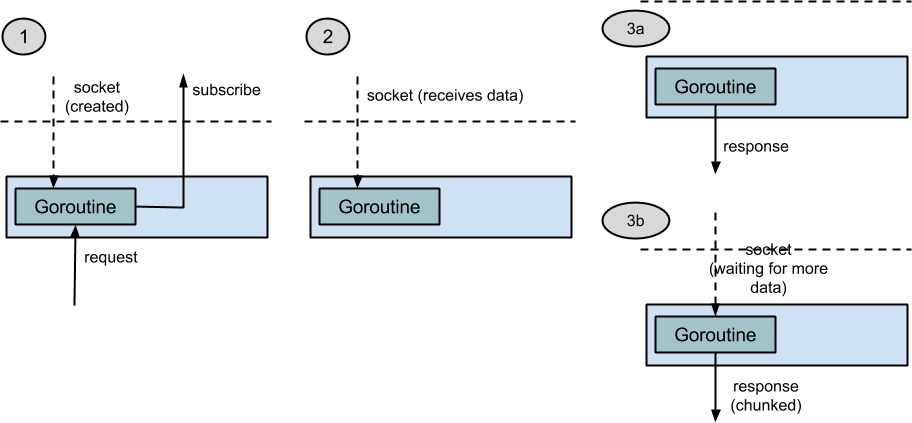
\includegraphics[scale=0.6]{implementation/images/api.png}
  \caption{The life cycle of a Request}\label{fig:api}
\end{figure}
